\chapter{Diseño del sistema.}
\label{cap: capitulo_4}

Durante el presente capítulo se expondrán los procedimientos de diseño \textit{hardware} e implementación \textit{software} la PCB que controlará nuestro horno.

En esta sección se analizaran las soluciones tomadas para cumplir los requisitos propuestos en el capítulo \ref{cap:capitulo_2}.


\section{Implementación \textit{Hardware}}

A la hora de diseñar la parte \textit{hardware} hemos de tener en cuenta las distintas partes de las que constará nuestro sistema para su correcto funcionamiento.

\begin{itemize}
	\item  Control y procesamiento: Hay que seleccionar la solución óptima en el control y
procesamiento de forma que tenga la capacidad de llevar a cabo toda la funcionalidad,
y que sea una solución robusta y del menor coste posible.
	\item  Sistemas de medida de temperatura: Se precisa buscar la manera de medir la temperatura de la manera más precisa posible y teniendo en cuenta los rangos de temperatura en los que trabaja el horno(0-300$^{\circ}C$).
	\item  Elección de los componentes: Se tomarán las decisiones para elegir la solución más adecuada entre las posibilidades planteadas anteriormente.
	
\end{itemize}



\subsection{Control y procesamiento}
El control y procesamiento es la parte más importante a nivel \textit{hardware}. Es por ello que debemos empezar por aquí. El resto de apartados dependerán de nuestra elección.

Para este proyecto se precisa un dispositivo fácil de programar, lo más barato posible, compatible con distintos componentes externos y con un módulo de conversores A/D. 

Aunque la mejor opción hubiera sido el uso de un PIC, porque nos permite diseñar un sistema a la medida de nuestras necesidades. Debido al poco tiempo del que disponía, se opto por usar un Arduino UNO.   
\begin{itemize}
	\item Open Source: Arduino es una plataforma de código y hardware abierto, es decir, puedes acceder a todo aspecto del funcionamiento circuital y algorítmico de las placas, y mucho mejor que eso, te dan todos los archivos Eagle, diagramas y componentes para que tu mismo crees tu versión de Arduino. 
	\item Fácil de programar: Arduino te ofrece un entorno de desarrollo integrado (IDE) con funciones preestablecidas que reducen la lógica a lectura de entradas, control de tiempos y salidas de una manera semántica e intuitiva.
	\item Documentación y tutoriales en exceso: Internet esta plagado literalmente de documentación sobre esta plataforma.
	\item Librerías: Una de las ventajas mas grandes que tiene Arduino es que poseen librerías para prácticamente cualquier componente externo que se le quiera acoplar. 
	\item Precio: Las placas de Arduino tienen un precio de entre 21\$ y 71\$, dependiendo del modelo que elijamos.
\end{itemize}


\subsection{Sistema de medida de temperatura}
Para la obtención de la temperatura se ha optado por el uso de sensores PT100. Consiste en un alambre de
platino que a 0 °C tiene 100 ohms y que al aumentar la temperatura aumenta su resistencia eléctrica. El incremento de la resistencia no es lineal pero si creciente y característico del platino de tal forma que mediante tablas(figura \ref{fig:tablaPT100}) es posible encontrar la temperatura exacta a la que corresponde.

\begin{figure}[H]%here
\noindent \begin{centering}
\includegraphics[scale=1.1]{capitulo4/tablaPT100}
\par\end{centering}
\caption{\label{fig:tablaPT100} Tabla de resistencias de una PT100.}
\smallskip
\end{figure}
Un Pt100 es un tipo particular de RTD (Dispositivo Termo Resistivo). Normálmente las Pt100 industriales se consiguen encapsuladas en la misma forma que las termocuplas, es decir dentro de un tubo de acero inoxidable ú otro material (vaina) , en un extremo está el elemento sensible (alambre de platino) y en el otro está el terminal eléctrico de los cables protejido dentro de una caja redonda de aluminio (cabezal). 
Las Pt100 siendo lévemente más costosos y mecánicamente no tán rígidos como las termocuplas, las superan
especiálmente en aplicaciones de bajas temperaturas (-100 a 200  $^{\circ}C$).
Los Pt100 pueden fácilmente entregar precisiones de una décima de grado con la ventaja que la Pt100 no se descompone graduálmente entregando lecturas erroneas, si no que normálmente se abre, con lo cual el dispositivo medidor detecta inmediátamente la falla del sensor y da aviso. 

Existen 3 modos de conexión para las Pt100, cada uno de ellos requiere un instrumento lector distinto.
El objetivo es determinar exactamente la resistencia electrica R(t) del elemento sensor de platino sín que influya en la lectura la resistencia de los cables Rc. En nuestro caso usaremos una PT100 de 4 hilos.

El método de 4 hilos es el más preciso de todos, los 4 cables pueden ser distintos (distinta resistencia) pero el instrumento lector es más costoso.

\begin{figure}[H]%here
\noindent \begin{centering}
\includegraphics[scale=0.6]{capitulo4/PT100_4hilos}
\par\end{centering}
\caption{\label{fig:PT100_4hilos} Conexión de una PT100 de 4 hilos.}
\smallskip
\end{figure}

Por los cables 1 y 4 se hace circular una corriente I conocida a traves de R(t) provocando una diferencia de potencial V en los extremos de R(t). Los cables 2 y 4 están conectados a la entrada de un voltímetro de alta impedancia luego por estos cables no circula corriente y por lo tanto la caida de potencial en los cables Rc2 y Rc3 será cero (dV=Ic*Rc=0*Rc=0) y el voltímetro medirá exáctamente el voltaje V en los extremos del elemento R(t). Finalmente el instrumento obtiene R(t) al dividir V medido entre la corriente I conocida.

La corriente I conocida se consigue mediante una fuente de corriente constante que se detellará en el apartado \ref{sec:BC}

\subsection{Elección de componentes}

En este apartado se seleccionarán los dispositivos que usaremos para el correcto funcionamiento de nuestra PCB y así conseguir cumplir los requisitos propuestos.

Se intentaran buscar los dispositivos más baratos, de menor consumo posible y a ser posible con montaje superficial \acrshort{SMD} (\acrlong{SMD}).

Los distintos dispositivos y componentes seleccionados son los siguientes:

\begin{itemize}
	\item Arduino UNO
	\item Display \glsname{LCD} 4x20A 
	\item Regulador de voltaje LM7805
	\item Transistor PNP BC857
	\item Rotary Encoder 
	\item Optotriac MOC3061M
	\item Triac BT139
\end{itemize}

\subsubsection{Arduinio UNO}
Se optó por usar un Arduino UNO \cite{Arduino}, ya que cubría todas nuestras necesidades y era uno de los modelos más baratos. 

Arduino es una placa con un microcontrolador de la marca Atmel, el ATMega328 \cite{ATMega}, y con toda la circuitería de soporte, que incluye, reguladores de tensión, un puerto USB (En los últimos modelos, aunque el original utilizaba un puerto serie) conectado a un módulo adaptador USB-Serie que permite programar el microcontrolador desde cualquier PC de manera cómoda y también hacer pruebas de comunicación con el propio chip.
Un arduino dispone de 14 pines que pueden configurarse como entrada o salida y a los que puede conectarse cualquier dispositivo que sea capaz de transmitir o recibir señales digitales de 0 y 5 V.
También dispone de entradas y salidas analógicas. Mediante las entradas analógicas podemos obtener datos de sensores en forma de variaciones continuas de un voltaje. Las salidas analógicas suelen utilizarse para enviar señales de control en forma de señales \acrshort{PWM}.

\smallskip
\begin{figure}[H]%here
\noindent \begin{centering}
\includegraphics[scale=0.2]{capitulo4/ArduinoUno}
\par\end{centering}
\caption{\label{fig:ArduinoUno} Vista frontal de Arduino UNO .}
\end{figure}
\smallskip

A continuación expondremos el mapeado de pines del Arduino UNO, disponible en la página web de Arduino \cite{Arduino}.


\smallskip
\begin{figure}[H]%here
\noindent \begin{centering}
\includegraphics[scale=1]{capitulo4/ARDUINOPINMAP}
\par\end{centering}
\caption{\label{fig:ARDUINOPINMAP} Arduino UNO pin mapping.}
\end{figure}
\smallskip



\subsubsection{Display \glsname{LCD} 4x20A}

Este pantalla \glsname{LCD} funciona basándose en el estándar de display 4x20 caracteres, y será configurado, su funcionamiento, por software. El único hardware adicional de adaptación que requiere es únicamente un potenciómetro que establezca el nivel de contraste de la pantalla.

\hfill
\begin{figure}[H]%here
\noindent \begin{centering}
\includegraphics[scale=0.5]{capitulo4/LCD}
\par\end{centering}
\caption{\label{fig:LCD} Display LCD 4x20 204A.}
\end{figure}
\hfill

Las principales características de nuestra \glsname{LCD} \cite{LCD} son: 

\smallskip
\begin{figure}[H]%here
\noindent \begin{centering}
\includegraphics[scale=0.9]{capitulo4/caracteristicas_lcd}
\par\end{centering}
\caption{\label{fig:caracteristicas_lcd} Principales características del Display LCD 4x20 204A.}
\end{figure}
\smallskip

Para el correcto funcionamiento del BackLight se tuvo que introduciendo una resistencia en la parte trasera de nuestra \glsname{LCD}. Para el cálculo de esta resistencia se tienen en cuenta los siguientes datos: alimentamos nuestra \glsname{LCD} con 5V, el Forward Voltage es de 3.2V y la corriente máxima es de 30mA. Por lo que nuestra resistencia se calcula de la siguiente manera:

\begin{equation}
R\geq(\frac{(5-3.2)V}{30mA})=60 \Omega
\end{equation}

Finalmente cogimos una resistencia de 100 \Omega para nuestra \glsname{LCD}.


\subsubsection{Regulador de voltaje LM7805}
El regulador de voltaje LM7805 \cite{7805} entrega 5V de tensión continua. La tensión de alimentación debe ser un poco más de 2 voltios superior a la tensión que entrega el regulador y menor a 35V. Usualmente, el modelo estándar soporta corrientes de hasta 1 A aunque hay diversos modelos en el mercado con corrientes que van desde los 0,1A. El dispositivo posee como protección un limitador de corriente por cortocircuito, y además, otro limitador por temperatura que puede reducir el nivel de corriente.
El regulador de voltaje LM7805 lo usaremos para alimentar el Arduino con 5V. 

Ya que lo usamos para regular tensión proveniente de una una fuente de alimentación(en nuestro caso con un adaptador AC de una PSP), tendremos que hacer un filtrado para eliminar cualquier fluctuación de voltaje que pueda ocurrir. Para dicho filtrado colocaremos un condensador a la salida del regulador y dos a la entrada. Tal y como se muestra en la siguiente imagen:

\smallskip
\begin{figure}[H]%here
\noindent \begin{centering}
\includegraphics[scale=0.7]{capitulo4/regulador}
\par\end{centering}
\caption{\label{fig:regulador} Configuración del regulador de voltaje 7805.}
\end{figure}
\hfill

Los condensadores C2 y C3 seran no polarizados. Mientras que el condensador C1 será polarizado de al menos 16V para soportar los 12V.

Con esta configuración ya podemos alimentar nuestro Arduino UNO con 5V.

\subsubsection{Transistor PNP BC857}
\label{sec:BC}
A la hora de diseñar una fuente de corriente constante necesité de dos transistores \glsname{PNP}. Se buscó un transistor pequeño y barato. Los transistores PNP BC857 son la versión \acrshort{SMD} (\acrlong{SMD}) de los BC557 y su precio está entre 0.03\textup{\euro} y 0.1\textup{\euro} lal unidad según la cantidad que compremos.

\hfill
\begin{figure}[H]%here
\noindent \begin{centering}
\includegraphics[scale=0.2]{capitulo4/BC857}
\par\end{centering}
\caption{\label{fig:BC857} Transistor \glsname{PNP} BC857.}
\end{figure}
\hfill

Las principales características de este transistor \cite{BC857} son:

\hfill
\begin{figure}[H]%here
\noindent \begin{centering}
\includegraphics[scale=0.9]{capitulo4/tabla_BC}
\par\end{centering}
\caption{\label{tabla_BC} Características del BC857\cite{BC857}.}
\end{figure}
\hfill


La curva de ganancia de DC es la siguiente, figura \ref{fig:curva_BC}.

\hfill
\begin{figure}[H]%here
\noindent \begin{centering}
\includegraphics[scale=0.7]{capitulo4/curva_BC}
\par\end{centering}
\caption{\label{fig:curva_BC} Curva de ganancia de corriente en DC.}
\end{figure}
\hfill


Este transistor lo usaremos para crear una fuente de corriente constante. El esquema del circuito es el siguiente: 

\smallskip
\begin{figure}[H]%here
\noindent \begin{centering}
\includegraphics[scale=0.7]{capitulo4/fuente}
\par\end{centering}
\caption{\label{fuente} Esquema de una fuente de corriente constante.}
\end{figure}
\smallskip



\subsubsection{Rotary Encoder}
Los Rotary Encoder son dispositivos para medir ángulos. Se usan para medir de manera precisa la rotación de motores o para crear un controlador tipo rueda(knobs) que pueden girar indefinidamente. Algunos están equipados con un pulsador. Los Rotary cuentan con tres patillas: dos de salida y una que va a masa.


\hfill
\begin{figure}[H]%here
\noindent \begin{centering}
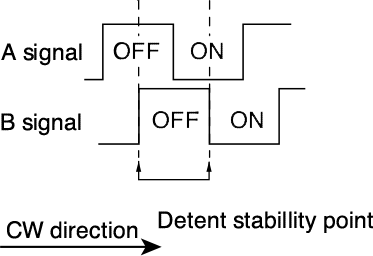
\includegraphics[scale=0.3]{capitulo4/rotary}
\par\end{centering}
\caption{\label{fig:rotary} Rotary Encoder.}
\end{figure}
\smallskip
	

El funcionamiento del Rotary Encoder se basa en que tenemos dos señales de salida cuadradas(A y B) que están desfasadas 90º. El número de pasos por vuelta variará según el modelo, en nuestro caso son 24. El siguiente diagrama muestra como las fases de A y B se relacionan según giremos el Rotary Encoder en el sentido de las agujas del reloj o en sentido contrario.

\smallskip
\begin{figure}[H]%here
\noindent \begin{centering}
\includegraphics[scale=0.8]{capitulo4/rotary_encoder_phase}
\par\end{centering}
\caption{\label{fig:rotary_encoder_phase} Relación de las señales A y B según el sentido del giro.}
\end{figure}
\smallskip

Cada vez que el pulso de la señal A va de positivo a cero, leemos el valor del pulso B. Podemos observar que cuando el Rotary Encoder se gira en el sentido de las agujas del reloj, B es siempre positivo. Mientras que si lo giramos en sentido contrario, B siempre es cero.

En nuestro proyecto hemos elegido uno tipo knob sin pulsador. Su conexión es muy simple, unicamente hay que conectar la patilla central a tierra y las otras dos a los pines 2 y 3 del Arduino, ya que son las habilitadas para interrupciones externas. 
La función del Rotary Encoder será la de permitirnos movernos por el menú y también poder establecer la temperatura de consigna que queramos.


\subsubsection{Optotriac MOC3061M}
Los triacs acoplados ópticamente combinan un diodo emisor de luz (\acrshort{led}) con un triac foto-detector (foto-triac) dentro de un mismo encapsulado con un esquema que es mostrado en la figura \ref{fig:optotriacs}. Al no existir conexión eléctrica entre la entrada y la salida, el acoplo es unidireccional (\acrshort{led} al foto-TRIAC) y permite un aislamiento eléctrico entre ambos dispositivos de hasta 7500 V (typ). Además, algunos foto-TRIAC incluyen un circuito de detección de paso por cero que permite sincronizar señales de la red eléctrica con señales de control del \acrshort{led} para ajustar el ángulo de conducción. 

\hfill
\begin{figure}[H]%here
\noindent \begin{centering}
\includegraphics[scale=0.8]{capitulo4/optotriacs}
\par\end{centering}
\caption{\label{fig:optotriacs} Esquema de un Optotriac.}
\end{figure}
\hfill

A continuación podemos ver las diferentes características de cada uno de los componentes del MOC3061M \cite{moc}.

\hfill
\begin{figure}[H]%here
\noindent \begin{centering}
\includegraphics[scale=1]{capitulo4/moc}
\par\end{centering}
\caption{\label{fig:moc} Características individuales de los componentes de un MOC306XM.}
\end{figure}
\hfill

En nuestro caso usamos el optotriac para aislar la etapa de control(circuitería de baja tensión) con la de potencia(la red y la carga) y de esta forma, evitar posibles daños en el Arduino UNO. Utilizamos un Optotriac MOC3061M, un optotriac con conmutación en el paso por cero y aislamiento entre entrada y salida. 

A continuación podemos ver las diferentes características de cada uno de los componentes 

A continuación, la figura \ref{fig:circuito_potencia} muestra la configuración usada en la etapa de potencia que controlara el encendido y apagado de nuestro horno. Donde la resistencia de 39 ohmios y el condensador de 0.1 microfaradios se usan para desairar el triac y a menudo, pero no siempre, necesario dependiendo del triac y de la carga.


\smallskip
\begin{figure}[H]%here
\noindent \begin{centering}
\includegraphics[scale=1]{capitulo4/circuito_potencia}
\par\end{centering}
\caption{\label{fig:circuito_potencia} Esquema de un Optotriac.}
\end{figure}
\smallskip





\subsubsection{Triac BT139}
El triac es un semiconductor, de la familia de los transistores. La diferencia con el tiristor convencional es que éste es unidireccional, es decir, funciona con corriente alterna en el sentido de polarización con medio semiciclo, y el triac es bidireccional, funciona en los semiciclos positivos y negativos. Cuando el triac conduce, hay una trayectoria de flujo de la polaridad del voltaje externo aplicado. Cuando el voltaje es más positivo en T2, la corriente fluye de T2 a T1 en caso contrario 	fluye de T1 a T2. En ambos casos el triac se comporta como un interruptor cerrado. Cuando el triac deja de conducir no puede fluir corriente por los terminales sin importar la polaridad del voltaje externo aplicado, por tanto actua como un interruptor abierto.

\smallskip
\begin{figure}[H]%here
\noindent \begin{centering}
\includegraphics[scale=0.8]{capitulo4/triac}
\par\end{centering}
\caption{\label{fig:triac} Esquema de un triac \cite{BT139}.}
\end{figure}
\smallskip


Las características del triac BT139 las podemos encontrar en su datasheet \cite{BT139}. Las más importantes son:

\smallskip
\begin{figure}[H]%here
\noindent \begin{centering}
\includegraphics[scale=0.7]{capitulo4/resistencia_termica}
\par\end{centering}
\caption{\label{fig:resistencia_termica} Resistencia termica.}
\end{figure}
\smallskip


\smallskip
\begin{figure}[H]%here
\noindent \begin{centering}
\includegraphics[scale=0.7]{capitulo4/caracteristicas_estaticas}
\par\end{centering}
\caption{\label{fig:caracteristicas_estaticas} Caracteristicas estaticas.}
\end{figure}
\smallskip

\smallskip
\begin{figure}[H]%here
\noindent \begin{centering}
\includegraphics[scale=0.7]{capitulo4/caracteristicas_dinamicas}
\par\end{centering}
\caption{\label{fig:caracteristicas_dinamicas} Caracteristicas dinamicas.}
\end{figure}
\smallskip






\subsection{Esquemático Altium}
En este apartado expondremos el diseño esquemático en el que juntaremos los distintos módulos ya interconectados. Se divide en dos: uno en el que se muestra los periféricos de control(LCD, pulsador, rotary y leds de control) y otro en el que se muestra la circuitería de control.

\subsection{Esquemático Altium}

\includepdf[pages=1,link=true,landscape,linkname=schematic,addtotoc={1,section,1,Esquemático Altium,letter}]{capitulo4/esquematico1}

\subsection{Esquemático Altium}
\includepdf[pages=1,link=true,landscape,linkname=schematic,addtotoc={1,section,1,Esquemático Altium,letter}]{capitulo4/esquematico2}



\section{Implementación \textit{Firmware}}
\label{sec:ImpFirm}


En este apartado se expondrán los distintos programas usados a lo largo del poryecto y su uso.

Principalmente se han usado tres programas: 



\begin{enumerate}
	\item ALTIUM \textit{Designer} versión 14.1: Con este \textit{software}, a partir del circuito esquemático se obtendrá la correspondencia en circuito \acrshort{PCB}. 
	\item Arduino IDE versión 1.0.6: Este \textit{software} lo podemos encontrar en la página de arduino. Es un  \textit{software} libre y muy sencillo de usar. Con él programaremos la rutina principal para el control de nuestro horno.
	\item MATLAB R2013a: Gracias a su gran procesamiento de datos, podremos representar los datos obtenidos de la temperatura dentro del horno y representarlos para poder obtener conclusiones sobre el comportamiento de nuestro horno.
\end{enumerate}

\subsection{ALTIUM \textit{Designer}}
Altium Designer es una solución integrada de hardware y software para cubrir todas las etapas de un desarrollo que van desde después de la idea hasta el prototipo final.

Altium Designer es un recurso para el diseño electrónico en todas sus fases y para todas las disciplinas, ya sean esquemas, simulación, diseño de circuitos impresos, imple¬mentación de FPGA o desarrollo de código para microprocesadores.

 Detrás de lo que encierra el nombre Altium Designer existe una plataforma de integración de software que reúne todas las herramientas necesarias para crear un entorno completo para el desarrollo de productos electrónicos, en una sola aplicación. Altium Designer incluye herramientas para todas las tareas de diseño: desde la captura de diseño esquemático y HDL, simulación de circuitos, análisis de integridad de señales, diseño de \acrshort{PCB}, hasta el diseño de sistemas embebidos. Características de Altium Designer:

\begin{itemize}
	\item Diseño de \acrshort{PCB}:
Altium Designer ha unificado el diseño de la plataforma física con el diseño de tarjeta de circuito impreso, con soporte para lógica programable. Esto proporciona un sistema de desarrollo totalmente unificado que puede desplegarse a través de todos los elementos del proceso de diseño de productos electrónicos.
	\item Gestión de librerías:
Elegir un componente obsoleto o fuera de stock de puede dar lugar a la producción de largos retrasos y sobrecostos. Altium Designer ofrece una amplia gama de herramientas de gestión de datos y recursos de información que le permiten mantener el control sobre el uso de partes.
	\item Diseño para fabricación:
Altium Designer ayuda a reducir la brecha entre el diseño y la fabricación, ademas le permite administrar de forma activa la generación y verificación de todos los datos de fabricación, ahorrando tiempo y minimizando los costosos, errores durante el flujo de diseño.
	\item Dispositivos programables:
Altium Designer es la única herramienta que permite explotar plenamente el potencial que ofrecen hoy los dispositivos programables, al unificar el diseño de \acrshort{FPGA}s, el desarrollo de software y el diseño de \acrshort{PCB}s, en una sola plataforma.
	\item Diseño Unificado de \acrshort{FPGA}/\acrshort{PCB}:
Los dispositivos programables son cada vez más usados en desarrollo electrónico. Este tipo de dispositivos abren nuevas posibilidades de diseño y aportan beneficios significativos para el proceso de diseño, lo que permite que la complejidad funcional se traslade de dispositivos discretos cableados al ámbito de dispositivos programables.
	\item Gestión de todo el proceso de desarrollo:
Altium Designer unifica todo el proceso de diseño y permite gestionar todos los aspectos del desarrollo dentro de un único entorno de diseño, y ofrece una infraestructura de administración de proyectos y documentos unificada que soporta la convergencia de diseños de tradicionalmente disciplinas separadas.
	
\end{itemize}

\subsection{Arduino IDE}

Para programar la placa es necesario descargarse de la página web de Arduino el entorno de desarrollo (IDE). Se dispone de versiones para Windows y para MAC, así como las fuentes para compilarlas en LINUX.
Estructura básica de un programa

La estructura básica de programación de Arduino es bastante simple y divide la ejecución en dos partes: setup y loop. Setup() constituye la preparación del programa y loop() es la ejecución. En la función Setup() se incluye la declaración de variables y se trata de la primera función que se ejecuta en el programa. Esta función se ejecuta una única vez y es empleada para configurar el pinMode (p. ej. si un determinado pin digital es de entrada o salida) e inicializar la comunicación serie. La función loop() incluye el código a ser ejecutado continuamente (leyendo las entradas de la placa, salidas, etc.). 

\subsection{MATLAB}
MATLAB (abreviatura de MATrix LABoratory, "laboratorio de matrices") es una herramienta de software matemático que ofrece un entorno de desarrollo integrado (IDE) con un lenguaje de programación propio (lenguaje M) y servicio de especie. Está disponible para las plataformas Unix, Windows, Mac OS X y GNU/Linux .

Entre sus prestaciones básicas se hallan: la manipulación de matrices, la representación de datos y funciones, la implementación de algoritmos, la creación de interfaces de usuario (GUI) y la comunicación con programas en otros lenguajes y con otros dispositivos hardware. El paquete MATLAB dispone de dos herramientas adicionales que expanden sus prestaciones, a saber, Simulink (plataforma de simulación multidominio) y GUIDE (editor de interfaces de usuario - GUI). Además, se pueden ampliar las capacidades de MATLAB con las cajas de herramientas (toolboxes); y las de Simulink con los paquetes de bloques (blocksets).
